%% This is file `elsarticle-template-1-num.tex',
%% %% Copyright 2009 Elsevier Ltd
%%
%% This file is part of the 'Elsarticle Bundle'.
%% ---------------------------------------------
%%
%% It may be distributed under the conditions of the LaTeX Project Public
%% License, either version 1.2 of this license or (at your option) any
%% later version.  The latest version of this license is in
%%    http://www.latex-project.org/lppl.txt
%% and version 1.2 or later is part of all distributions of LaTeX
%% version 1999/12/01 or later.
%%
%% The list of all files belonging to the 'Elsarticle Bundle' is
%% given in the file `manifest.txt'.
%%
%% Template article for Elsevier's document class `elsarticle'
%% with numbered style bibliographic references
%%
%% $Id: elsarticle-template-1-num.tex 149 2009-10-08 05:01:15Z rishi $
%% $URL: http://lenova.river-valley.com/svn/elsbst/trunk/elsarticle-template-1-num.tex $
%%

\documentclass[preprint,5p,times,twocolumn]{elsarticle}
%\documentclass[final,5p,times,twocolumn]{elsarticle}

%% Use the option review to obtain double line spacing
%% \documentclass[preprint,review,12pt]{elsarticle}

%% Use the options 1p,twocolumn; 3p; 3p,twocolumn; 5p; or 5p,twocolumn
%% for a journal layout:
%% \documentclass[final,1p,times]{elsarticle}
%% \documentclass[final,1p,times,twocolumn]{elsarticle}
%% \documentclass[final,3p,times]{elsarticle}
%% \documentclass[final,3p,times,twocolumn]{elsarticle}
%% \documentclass[final,5p,times]{elsarticle}
%% \documentclass[final,5p,times,twocolumn]{elsarticle}

%% if you use PostScript figures in your article
%% use the graphics package for simple commands
%% \usepackage{graphics}
%% or use the graphicx package for more complicated commands
%% \usepackage{graphicx}
%% or use the epsfig package if you prefer to use the old commands
%% \usepackage{epsfig}

%% The amssymb package provides various useful mathematical symbols
\usepackage{amssymb}

\usepackage{tikz}
\usetikzlibrary{shapes, arrows}


%% Styles for proximity flow chart
\tikzstyle{bcell} = [rectangle, draw, fill=red!20, minimum width=3em, text centered, minimum height=3em]
\tikzstyle{dcell} = [rectangle, draw, fill=yellow!20, minimum width=3em, text centered, minimum height=3em]
\tikzstyle{ecell} = [rectangle, draw, fill=black!20, minimum width=3em, text centered, minimum height=3em]
\tikzstyle{fcell} = [rectangle, draw, fill=green!20, minimum width=3em, text centered, minimum height=3em]
\tikzstyle{ucell} = [rectangle, draw, fill=white!20, minimum width=3em, text centered, minimum height=3em]
\tikzstyle{wcell} = [rectangle, draw, fill=blue!20, minimum width=3em, text centered, minimum height=3em]
\tikzstyle{line} = [draw, -latex']


\journal{University of Guelph; CIS*4780}

\begin{document}

\begin{frontmatter}

\title{Two Dimensional Intelligent Character Recognition; A Rope Of Sand}

%% use optional labels to link authors explicitly to addresses:
%% \author[label1,label2]{<author name>}
%% \address[label1]{<address>}
%% \address[label2]{<address>}

\author[ryan,doug,oliver]{Ryan Pattison, Douglas Anderson, and Oliver Cook}

\address[ryan]{ryan.m.pattison@gmail.com}
\address[doug]{dander01@guelph.ca}
\address[oliver]{cooko@uoguelph.ca}
 
\begin{abstract}
%% Text of abstract

For quite some time computer vision has been used to extract characters from
images in order to gain knowledge from text. In recent years many of the
techniques for recognizing characters has been based on machine learning.

\end{abstract}

\begin{keyword}
%% keywords here, in the form: keyword \sep keyword
Machine Learning \sep Data Mining \sep Computer Vision
%% MSC codes here, in the form: \MSC code \sep code
%% or \MSC[2008] code \sep code (2000 is the default)

\end{keyword}

\end{frontmatter}

%%
%% Start line numbering here if you want
%%
%%\linenumbers

%% main text
\section{Introduction}
\label{intro}
Lorem ipsum dolor sit amet, consectetur adipiscing elit. Morbi at nulla eu
turpis posuere imperdiet eget id nibh. Mauris eget orci et dui lobortis
malesuada. Aliquam a purus convallis, consequat libero eu, molestie leo.
Aliquam venenatis massa sit amet erat viverra elementum. Morbi varius magna eu
imperdiet volutpat. Cras suscipit mi sed ultrices tempus. Fusce ullamcorper
magna in euismod vehicula.


Nunc placerat porttitor tortor, vel tristique erat lacinia eget. Suspendisse a
sodales urna, sit amet congue felis. Quisque convallis posuere arcu. Sed mollis
mauris eget imperdiet tincidunt. Aenean malesuada ultricies lacinia. Vivamus
pharetra in massa suscipit tristique. Mauris vitae vulputate diam. Cras ac leo
sed odio fringilla aliquam. Fusce vehicula feugiat quam in laoreet. Nam
facilisis enim ac justo lacinia, ac ullamcorper nulla ornare. Phasellus ligula
mauris, aliquam ultrices ultrices id, rutrum vitae elit. Nunc eget sapien vel
tellus pretium adipiscing. Fusce elit tortor, sagittis sit amet cursus eu,
blandit ac diam. Phasellus posuere, mauris at mattis consequat, nulla dolor
dapibus tortor, ut consectetur quam tortor vitae justo.

\section{Process}
\label{process}

\subsection{Overview}
\label{process:overview}
rem ipsum dolor sit amet, consectetur adipiscing elit. Morbi sodales lobortis
enim quis iaculis. Mauris ut dignissim metus, id rhoncus ligula. Nulla at odio
non turpis condimentum cursus vel eu leo. Morbi hendrerit venenatis vehicula.
Aliquam id condimentum metus. Duis rhoncus convallis fringilla. Suspendisse vel
ornare libero, sit amet ultricies mi. Suspendisse at justo odio. Morbi id
fringilla dui, quis pretium diam. Vivamus nisi est, varius vitae ipsum iaculis,
tincidunt pellentesque metus.

Duis pulvinar est a nisl euismod, in dapibus ante scelerisque. Pellentesque
tristique turpis eget ante tincidunt bibendum. Proin id arcu commodo, auctor
odio sit amet, aliquam nisi. Donec sem diam, iaculis sed justo ut, lacinia
consequat augue. In vitae semper ante. Nunc vitae lobortis odio. Nunc
condimentum nec mi eu suscipit. Morbi tempus orci semper condimentum consequat.
Aliquam erat volutpat. Sed id ipsum ut felis varius placerat vitae elementum
purus. Etiam ut ornare neque. Pellentesque dictum tellus dapibus metus
pharetra, vitae suscipit lectus ultricies. In varius augue ac lacinia viverra.

\subsection{Feature-Based Approach}
\label{process:featurebased}

Cras condimentum mauris at dolor faucibus ornare. Sed eu mauris id ipsum
vehicula pharetra. Pellentesque laoreet tempor volutpat. Nulla dapibus sodales
q
blandit. Curabitur vel dui ante. Interdum et malesuada fames ac ante ipsum
primis in faucibus. Nullam vestibulum leo orci, vitae sagittis massa blandit
quis. Integer venenatis urna ut urna ornare lacinia. Nam semper, leo non
convallis suscipit, diam tortor viverra justo, vel semper libero justo sit amet
purus. Aenean sodales elit sed velit auctor fringilla. In consectetur, elit sit
amet consectetur auctor, libero nisl dictum justo, nec dapibus arcu elit vitae
diam.

\subsection{Gold Comparison Approach}
\label{process:gold}

Lorem ipsum dolor sit amet, consectetur adipiscing elit. Praesent sit amet
adipiscing erat. Nulla at elit mollis, faucibus tellus et, molestie sem. Aenean
imperdiet consequat faucibus. Nullam felis libero, ultricies eget augue at,
suscipit pellentesque arcu. Praesent quis metus quis neque aliquet commodo. Sed
eget bibendum tortor, tempus venenatis ipsum. Vivamus eget lectus vitae lorem
commodo elementum. Etiam felis lorem, tempus ac vulputate in, vulputate vel
neque. Nullam euismod ligula eu tortor mattis lobortis. Vivamus luctus, mi
laoreet hendrerit rutrum, quam dolor viverra odio, vitae adipiscing mi justo a
nunc.

Pellentesque malesuada, purus at tempor venenatis, dolor nisi posuere velit, et
gravida velit magna sit amet eros. Quisque sagittis, eros in convallis aliquam,
velit felis auctor arcu, at cursus ligula diam sit amet lacus. Suspendisse in
tortor sed augue convallis lacinia sit amet eu est. Duis quis urna in nulla
gravida pellentesque aliquam eleifend eros. Phasellus tristique, neque vel
pretium congue, justo felis vestibulum metus, at mollis lorem dolor quis
lectus. Maecenas vel feugiat tellus. Suspendisse nisi tellus, cursus ultricies
lectus et, dictum pretium purus. Fusce a vestibulum lectus. Nulla varius
suscipit egestas. Curabitur magna lectus, interdum a lorem vel, sodales
suscipit dolor. Phasellus rutrum eros a metus ornare tempor. Quisque id lorem
eu erat tempus viverra ac vitae lectus. Aliquam ullamcorper, ipsum in tincidunt
ullamcorper, lacus eros mollis neque, eu pharetra mauris magna sit amet magna.
Integer nunc orci, varius fringilla fermentum ornare, aliquam ac erat. Fusce eu
sapien pharetra, lobortis risus nec, sodales felis. Aliquam sed faucibus est.

\subsection{Proximity Approach}
\label{process:proximity}

Summary of approach

\begin{center}
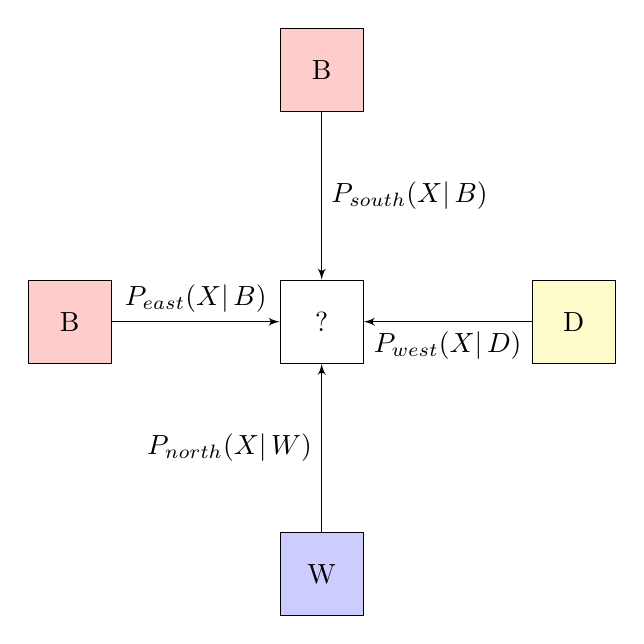
\begin{tikzpicture}[node distance = 3.2 cm, auto]
    \node[bcell](top){B};
    \node[ucell, below of=top](center){?};
    \node[bcell, left of=center](left){B};
    \node[dcell, right of=center](right){D};
    \node[wcell, below of=center](bottom){W};

    \path[line] (top)   -- node {$P_{south}(X | \, B)$} (center);

    \path[line] (left)  -- node {$P_{east}(X | \, B)$} (center);
    \path[line] (right) -- node {$P_{west}(X | \, D)$} (center);
    \path[line] (bottom) -- node {$P_{north}(X | \, W)$} (center);
\end{tikzpicture}
\end{center}

Let $V_{d}$ be a vector of probabilities, where $n$ is the number of classes,
$d$ is a direction.

\begin{equation}
V_{d} = \{P_{d}{(X_{1} | \, C_{d})}, P_{d}{(X_{2} | \, C_{d}),\; \ldots \; , P_{d}{(X_{n}) | \, C_{d}}}\}
\end{equation}

 To determine the probability of a cell being in a particular class
we can multiply the vectors of all directions together using the scalar
product.

\begin{equation}
C = V_{north} \cdot V_{east} \cdot V_{south} \cdot V_{west}
\end{equation}

This new vector $C$ will contain $n$ probabilities that this cell should be
classified a particular class. Since the vectors were multiplied together the
range of the values in $C$ is no longer $\in[0,1]$. We can select the maximum
value in $C$ to choose a class.

An example of this process can be seen with the following situation:

\begin{center}
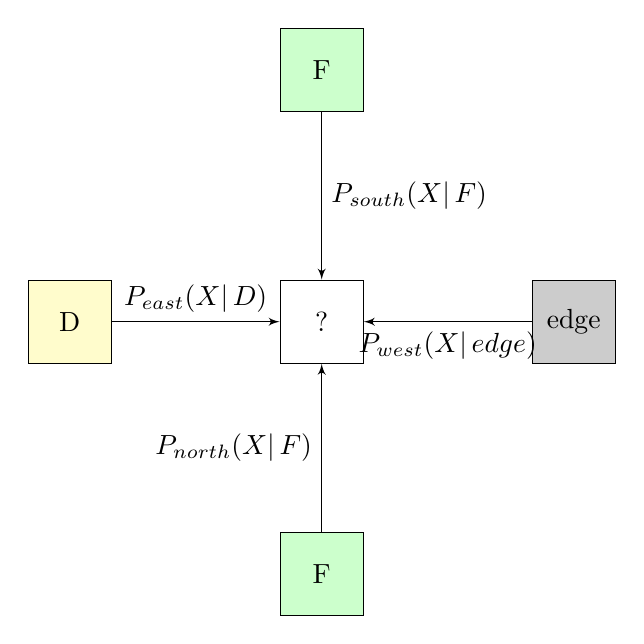
\begin{tikzpicture}[node distance = 3.2 cm, auto]
    \node[fcell](top){F};
    \node[ucell, below of=top](center){?};
    \node[dcell, left of=center](left){D};
    \node[ecell, right of=center](right){edge};
    \node[fcell, below of=center](bottom){F};

    \path[line] (top)   -- node {$P_{south}(X | \, F)$} (center);
    \path[line] (left)  -- node {$P_{east}(X | \, D)$} (center);
    \path[line] (right) -- node {$P_{west}(X | \, edge)$} (center);
    \path[line] (bottom) -- node {$P_{north}(X | \, F)$} (center);
\end{tikzpicture}
\end{center}

Suppose that the training set has the following characteristics:

\begin{table}
\begin{tabular}{ l c r }
    class & $x_{0}$ & $x_{1}$ \\
    north & 2 & 3 \\
    east  & 8 & 9 \\
    south & 5 & 6 \\
    west  & 5 & 6 \\
\end{tabular}
\caption{The probability data is...} %TODO
\end{table}

Quisque viverra pretium urna et pharetra. Nunc facilisis, justo vel luctus
convallis, dolor tortor varius diam, eget semper massa arcu eu tortor. Duis a
nibh mauris. Suspendisse facilisis erat ultricies fermentum adipiscing. Aliquam
erat volutpat. Proin blandit mauris nec justo fringilla, consectetur hendrerit
augue interdum. Pellentesque habitant morbi tristique senectus et netus et
malesuada fames ac turpis egestas. Aenean viverra augue diam, eu laoreet dolor
tristique eget. Nam fringilla lectus sem, sed aliquet ante dictum vel. Vivamus
nec pellentesque dolor. Pellentesque condimentum augue dui, ut mattis est
blandit at.

\subsection{Classifier Training}
\label{process:training}

To gain knowledge from the data that we have just generated we use the software tool WEKA\cite{Hall2009}.

Lorem ipsum dolor sit amet, consectetur adipiscing elit. Morbi sed eros tortor.
Suspendisse a ipsum vehicula, hendrerit eros eget, venenatis orci. In sed
placerat dolor. Donec suscipit, ante in varius interdum, lorem metus vestibulum
ligula, ac luctus libero diam quis nisl. Maecenas eu nisi sed magna egestas
lobortis. Quisque accumsan fermentum lorem sed vehicula. In at nulla gravida,
ultricies sapien nec, ornare nulla. Nunc arcu nunc, mollis in augue sit amet,
blandit gravida lacus. Cras posuere laoreet tellus a aliquam. In eleifend
molestie sapien, vitae euismod eros commodo id.

Sed varius consequat nulla, eget pulvinar metus suscipit vel. Etiam accumsan
condimentum neque, a tincidunt ipsum laoreet id. Nunc fermentum hendrerit nulla
et sagittis. Sed varius nisl porta, posuere enim blandit, fringilla sem. In non
velit ultrices, mattis eros sit amet, lobortis tortor. Morbi rhoncus vestibulum
eros quis bibendum. Aliquam at pretium ante. Ut quis sagittis orci, et pretium
leo. Quisque congue, lacus nec dictum lacinia, sem justo aliquet leo, ut
placerat orci lacus eu neque. In hac habitasse platea dictumst. Nulla non
posuere nisi, a iaculis sem.

\section{Results}
\label{results}

Praesent sagittis nisl ipsum, ut porta tortor suscipit in. Maecenas adipiscing
nisl eros, sed bibendum diam eleifend vitae. Donec quis leo convallis,
consequat odio nec, mattis arcu. Etiam et sem nulla. Quisque eu elit elit.
Curabitur quis mi quis dui tincidunt scelerisque in vitae lorem. Quisque nunc
ante, suscipit id dolor at, viverra volutpat augue. Curabitur non hendrerit
sapien. Quisque vestibulum ante bibendum felis ornare fermentum. Maecenas
fringilla fringilla ante vel elementum. Fusce diam turpis, commodo et interdum
eget, molestie nec eros. Vestibulum vel nibh cursus, sodales tellus eu, mattis
lacus. Quisque vestibulum nisi dui. Cras luctus, risus non pellentesque
pharetra, sem dui laoreet dolor, eu elementum neque risus id ante. Mauris
sagittis, tortor eu sodales condimentum, nibh lacus porta felis, sed feugiat mi
diam quis quam.

\subsection{Feature-Based Classifier}
\label{results:featurebased}

Lorem ipsum dolor sit amet, consectetur adipiscing elit. Curabitur non nisl
quis ipsum consequat interdum quis vitae risus. Sed pulvinar nunc eros, eget
pretium lorem luctus ut. Nulla consequat justo et mauris posuere suscipit. Sed
in nisl convallis, tristique nulla egestas, feugiat est. Ut consequat sed felis
vel convallis. Sed consectetur interdum mi a tristique. Maecenas placerat
laoreet augue, in auctor sem aliquam at. Nulla fermentum quam iaculis nisl
pulvinar, nec ultricies turpis ornare. Integer eu est in quam dignissim
scelerisque. Maecenas blandit viverra diam eu aliquet. Donec ac tellus id dolor
iaculis aliquet lobortis eu lorem.

Vivamus pretium lorem ac arcu adipiscing aliquet. Aliquam id orci pharetra
ipsum feugiat imperdiet. Vestibulum dolor nibh, lacinia eu vulputate ac,
consequat in enim. Suspendisse eu suscipit est. Donec porttitor euismod nisl,
et accumsan tellus egestas et. Morbi consectetur, diam id sollicitudin viverra,
felis tortor ullamcorper augue, et luctus leo metus vel ipsum. Cras eu placerat
purus. Fusce sollicitudin accumsan mi. Suspendisse potenti. Curabitur fermentum
nulla eget turpis scelerisque sodales. Donec hendrerit at turpis quis
ultricies. Vestibulum ante ipsum primis in faucibus orci luctus et ultrices
posuere cubilia Curae; Nullam sed magna nec tortor congue congue ut id lectus.
Sed sed venenatis neque. Nunc iaculis blandit sem nec aliquam. Aliquam blandit
quam ac neque venenatis, in tempor nisl porta.

\subsection{Gold Comparison Classifier}
\label{results:gold}

Lorem ipsum dolor sit amet, consectetur adipiscing elit. Cras metus nunc,
posuere et viverra mollis, faucibus quis odio. Praesent condimentum vestibulum
purus, in ultricies nibh tristique interdum. Praesent mi neque, convallis id
lectus ut, gravida tempus felis. Curabitur eget tortor cursus, placerat magna
ut, aliquet justo. Donec tortor magna, laoreet at urna eget, molestie imperdiet
est. Nullam lacinia mi felis, sed facilisis nisi ullamcorper et. Cras in
feugiat nulla, non congue felis. Aliquam pulvinar dignissim enim at sodales.
Pellentesque faucibus dignissim tellus, eu consequat purus suscipit vel. Donec
tristique luctus faucibus. Nulla facilisi.

Curabitur egestas lorem ullamcorper, tristique orci in, tempor nulla. Praesent
volutpat lorem purus. Quisque ultrices turpis non felis suscipit porta. Integer
libero leo, lacinia at egestas sed, tempus a libero. Proin tempus vulputate
commodo. Pellentesque eu iaculis libero. Ut id mauris mi.

\subsection{Proximity Classifier}
\label{results:proximity}

Lorem ipsum dolor sit amet, consectetur adipiscing elit. Fusce vitae eros id
urna convallis mattis. Donec suscipit nulla a accumsan tempor. Aenean vehicula
dapibus sem, sit amet aliquam quam porttitor vel. Vivamus nec neque at tortor
eleifend facilisis nec scelerisque lacus. Phasellus pellentesque odio eu tortor
lacinia suscipit. Donec in felis varius dui aliquam condimentum lacinia vel
arcu. Nullam lobortis magna ut tellus dignissim, non dictum odio mollis.

Donec ut lectus pretium, molestie enim et, aliquam metus. Vestibulum ante ipsum
primis in faucibus orci luctus et ultrices posuere cubilia Curae; Curabitur a
rutrum magna. Sed quis nisi ac felis molestie tempus et at orci. Aliquam vitae
neque sit amet odio imperdiet adipiscing. Fusce in ipsum a odio mollis mattis.
Fusce aliquet sed urna sit amet tempor. Donec elementum vestibulum turpis, sit
amet consequat lacus tempor eu. Pellentesque habitant morbi tristique senectus
et netus et malesuada fames ac turpis egestas. Etiam justo lectus, lobortis non
rhoncus ac, pulvinar vitae nulla. Nullam libero orci, ultrices ut faucibus in,
sagittis et dui. Nulla dui dui, porttitor nec leo

\section{Conclusions}
\label{conclusions}

Lorem ipsum dolor sit amet, consectetur adipiscing elit. Nulla nec rhoncus
enim, eu iaculis sapien. Vestibulum lobortis velit eu nunc condimentum viverra.
Donec nunc mi, condimentum sed vehicula ut, dignissim vitae erat. Nulla in
bibendum nunc, sed gravida arcu. Vestibulum eget laoreet eros. Praesent semper
ultrices nulla, ut molestie justo ultrices eget. Morbi a facilisis sem. Donec
et nunc felis. Ut consequat elit tellus, vitae feugiat dui posuere et. Mauris
adipiscing ipsum a faucibus laoreet. Nunc in cursus neque.

Aenean a tristique tortor. Donec porttitor dui nec quam tincidunt, quis rhoncus
nisi iaculis. Proin laoreet suscipit euismod. Nullam venenatis purus vitae nibh
venenatis, non tincidunt orci venenatis. Mauris ultrices diam ut libero
sagittis fringilla. Mauris tincidunt non diam nec consequat. Cras sed rutrum
lectus. Nulla tincidunt, metus ut lobortis condimentum, turpis nisi malesuada
sapien, sed bibendum diam sapien non velit. Aliquam eget leo eu ipsum feugiat
varius hendrerit eget massa.

Proin vel tortor id dui hendrerit pretium. Pellentesque quis suscipit risus, et
tempus sem. Ut at augue at urna pellentesque accumsan. Sed orci dui, pretium ac
pretium adipiscing, sagittis id nisl. Praesent a iaculis tellus, nec interdum
arcu. Nam est erat, varius sit amet nulla a, ultricies pellentesque sem.
Aliquam at enim nibh. In et luctus sapien. Nam venenatis venenatis tristique.

Etiam a massa non ipsum ullamcorper convallis. Nulla facilisi. Ut sed semper
mi. Quisque dignissim faucibus quam vitae hendrerit. Mauris quis rhoncus lorem,
non sagittis metus. Vestibulum fringilla est eu enim sodales semper. Curabitur
pharetra leo vel tortor ornare blandit. Suspendisse potenti. Curabitur pretium
in ligula quis molestie. Aenean sem lectus, hendrerit at aliquet posuere,
laoreet id felis. Integer pretium ipsum nec tempus placerat. Suspendisse ut
porta neque. Maecenas id molestie dolor, lacinia interdum quam.

\section{References}
\label{references}

%% The Appendices part is started with the command \appendix;
%% appendix sections are then done as normal sections
%% \appendix

%% \section{}
%% \label{}

%% References
%%
%% Following citation commands can be used in the body text:
%% Usage of \cite is as follows:
%%   \cite{key}          ==>>  [#]
%%   \cite[chap. 2]{key} ==>>  [#, chap. 2]
%%   \citet{key}         ==>>  Author [#]

%% References with bibTeX database:

\bibliographystyle{plain}
\bibliography{refs}

%% Authors are advised to submit their bibtex database files. They are
%% requested to list a bibtex style file in the manuscript if they do
%% not want to use model1-num-names.bst.

%% References without bibTeX database:

% \begin{thebibliography}{00}

%% \bibitem must have the following form:
%%   \bibitem{key}...
%%

% \bibitem{}

% \end{thebibliography}

\end{document}

